\documentclass[usepdftitle=false,aspectratio=169]{beamer}
\usepackage{amsmath, amsfonts, amssymb}
\usepackage{xspace}
\usepackage{xparse}
\usepackage[yyyymmdd]{datetime}
\usepackage{ulem}
\usepackage{array}
\usepackage{multirow}
\usepackage{booktabs}
\usepackage{stmaryrd}
\usepackage{subcaption}
\usepackage{bussproofs}
\usepackage{mathpartir}
\usepackage{minted}
\usemintedstyle{trac}

\usepackage{tikz}

\usetikzlibrary{shapes,arrows,positioning,decorations.markings,matrix,fit,calc}
\tikzstyle{line} = [draw, -latex']
\tikzstyle{rline} = [draw, latex'-]
\pgfdeclarelayer{background}
\pgfsetlayers{background,main}
\EnableBpAbbreviations

\hypersetup{
  pdftitle={Talk - Carcara: An efficient proof checker and elaborator for SMT
  proofs in the Alethe format - TACAS 2023},
  pdfauthor={Bruno Andreotti},
  pdfkeywords={},
  pdfborder={0 0 0}
  draft=false,
  bookmarksnumbered,
  bookmarksdepth=2,
  bookmarksopenlevel=2,
  bookmarksopen
}

\renewcommand{\dateseparator}{--}

%%% BEGIN Defining style
\useinnertheme[outline]{chamfered}
\setbeamertemplate{navigation symbols}{}%remove navigation symbols
\usefonttheme[onlymath]{serif}%beamer math looks like article math
\usecolortheme{seahorse}
\setbeamercolor{palette quinary}{use=structure,fg=black,bg=white}
%%% END Defining style

%%% BEGIN Biblatex for references
\usepackage[backend=bibtex,
doi=false,isbn=false,url=false,
% show initials only
style=alphabetic,
% Show name
% style=authoryear-icomp,
% citation label has 4 initials if up to 4 authors, 3 and "+" otherwise
maxalphanames= 4, maxcitenames = 3, minalphanames = 3, minnames = 3]{biblatex}
% citation label has first author's name et al
% maxcitenames=2,backend=biber]{biblatex}

\bibliography{./refs.bib}

%%%%%%%%%%%%% macros

\mathchardef\mhyphen="2D % Define a "math hyphen"

\usepackage{pifont}

\newcommand{\bluecheck}{{\color{blue}\checkmark}}
\newcommand{\redmark}{\color{red}{\ding{55}}}

\newcommand\vvthinspace{\kern+0.041667em}
\newcommand\vthinspace{\kern+0.083333em}
\newcommand\negvthinspace{\kern-0.083333em}
\newcommand\negvvthinspace{\kern-0.041667em}

\newcommand\FV[1]{\textrm{FV}(#1)}

\newcommand\sym[1]{\mathsf{#1}}

%ADT font macros
\newcommand{\typename}[1]{\mathbf{\mathrm{#1}}}
\newcommand{\consname}[1]{\mathrm{#1}}
\newcommand{\selname}[1]{\mathrm{#1}}
\newcommand{\testername}[1]{\mathrm{#1}}

\newcommand{\SInt}{\typename{Int}}
\newcommand{\SBool}{\typename{Bool}}
\newcommand{\SStr}{\typename{Str}}

\newcommand{\evalfn}[1]{\mathrm{eval}_{#1}}

\DeclareDocumentCommand{\qnt}{ O{n} m O{\psi}}{\innerqnt(#2,#1) #3}
\def\innerqnt(#1,#2,#3){#1 \bar #2.\>}

\DeclareDocumentCommand{\terms}{ m O{}}{\mathbf{T}_{#2}(#1)}

\DeclareDocumentCommand{\bfapp}{ O{f} m O{n}}{#1({\bar #2}_{#3})}
\DeclareDocumentCommand{\enum}{ O{n} m O{,\,} O{} O{1}}{#2_#5#4#3\dots #3#2_{#1}#4}
\DeclareDocumentCommand{\benum}{ O{n} m O{\mapsto} O{} O{,\,} O{1}}{\innerbenum(#2,#3,#6,#4)#5\dots #5\innerbenum(#2,#3,#1,#4)}
\def\innerbenum(#1,#2,#3,#4,#5){#1_{#4}#3 #5{#2_{#4}}}

\DeclareDocumentCommand{\bfenum}{O{\mapsto} m}{\innerbfenum(#2,#1)}
  \def\innerbfenum(#1,#2,#3){\bar #1#3 \bar #2}
\DeclareDocumentCommand{\fapp}{ O{f} m O{n} O{,\,} O{(} O{)}}{#1#5#2_1#4\dots #4#2_{#3}#6}

% Column that takes width (left justified): L{1cm}, e.g.
\newcolumntype{L}[1]{>{\raggedright\arraybackslash$} p{#1} <{$}}

% Column with math mode in displaystyle
\newcolumntype{F}[1]{>{$\displaystyle} #1 <{$}}

% Column with math mode in displaystyle
\newcolumntype{D}[1]{>{\displaystyle} #1 <{}}

% Allows to break like in cell; first arg is $t,b,c$, for alignment with other cells
\newcommand{\specialcell}[2][c]{%
  \begin{tabular}[#1]{@{}l@{}}#2\end{tabular}}

\newcommand{\ccfv}{\textsc{CCFV}}

% \newcommand{\cdclt}{CDCL($\mathcal{T}$)}
\newcommand{\cdclt}{CDCL(T)}
\newcommand{\dpllt}{\cdclt}

\newcommand{\cvcho}{\textsc{cvc}4-\textsc{ho}\xspace}
\newcommand{\cvc}{\textsc{cvc}4\xspace}
\newcommand{\zzz}{Z3}
\newcommand{\verit}{\textsc{veriT}\xspace}

\newcommand{\basestrat}[1]{{\bf #1}}
\newcommand\interleavestrat[2]{\basestrat{#1}+\basestrat{#2}}
\newcommand\mathinterleavestrat[2]{$\mathbf{#1}$+$\mathbf{#2}$}
\newcommand\prioritystrat[2]{\basestrat{#1};\basestrat{#2}}
\newcommand{\zbasestrat}[1]{{\bf z3 #1}}
\newcommand{\zprioritystrat}[2]{{\bf z3} \basestrat{#1};\basestrat{#2}}
\newcommand{\E}{\mathsf{E}}
\newcommand{\Q}{\mathsf{Q}}
\newcommand{\M}{\mathsf{M}}
\newcommand{\ite}{\mathsf{ite}}
\newcommand{\Mod}{\mathcal{M}}
\newcommand{\termordereq}{\preceq}
\newcommand{\termorder}{\prec}
\newcommand{\teq}{\simeq}
\newcommand{\tneq}{\not\simeq}

\newcommand{\inputform}{\psi}
\newcommand{\matrixform}{\varphi}

\newcommand\vitem{\vfill\item}
\newcommand\pvitem{\pause\vfill\item}
\newcommand\pitem{\pause\item}

\newcommand{\cvcsy}{\textsc{cvc}4\textsc{sy}\xspace}
\newcommand{\cvccegis}{\textsc{cvc+c}\xspace}
\newcommand{\cvcu}{\textsc{cvc+upi}\xspace}
\newcommand{\cvcuci}{\textsc{cvc+upi+e}\xspace}
\newcommand{\cvcport}{\textsc{cvc-port}\xspace}
\newcommand{\loopinv}{\textsc{loopinvgen}\xspace}

\newcommand{\divc}{D\&C\xspace}

% AJR : update these
\newcommand{\unif}{Unif+PI\xspace}
\newcommand{\unifci}{Unif+PI+E\xspace}
\newcommand{\smtclass}{\textsc{SMTClassify}\xspace}
\newcommand{\learn}{\textsc{Learn}\xspace}
\newcommand{\classchecker}{\textsc{ClassChecker}\xspace}

%%%%%%%%%%%%


% To avoid number in slides that break, like the references one
\setbeamertemplate{frametitle continuation}{}

% Small font
\renewcommand*{\bibfont}{\scriptsize}
%%% END Biblatex for references



%%% BEGIN DEFINING TITLE PAGE

\defbeamertemplate{title page}{mystyle}[1][]
{
  \vbox{}
  \vfill
  \begingroup
    \centering
    {\usebeamercolor[fg]{titlegraphic}\inserttitlegraphic\par}
    \vskip1em
    \begin{beamercolorbox}[sep=0pt,center,#1,rounded=true,wd=11cm]{title}
      \usebeamerfont{title}\inserttitle\par%
      \ifx\insertsubtitle\@empty%
      \else%
        \vskip0.25em%
        {\usebeamerfont{subtitle}\usebeamercolor[fg]{subtitle}\insertsubtitle\par}%
      \fi%
    \end{beamercolorbox}%
    \vskip1em\par
    \begin{beamercolorbox}[sep=8pt,center,#1]{author}
      \usebeamerfont{author}\insertauthor
    \end{beamercolorbox}
    \begin{beamercolorbox}[sep=8pt,center,#1]{institute}
      \usebeamerfont{institute}\insertinstitute
    \end{beamercolorbox}
    \begin{beamercolorbox}[sep=0pt,center,#1]{date}
      \usebeamerfont{date}\insertdate
    \end{beamercolorbox}%
  \endgroup
  \vfill
}

\setbeamertemplate{title page}[mystyle]

%%% END DEFINING TITLE PAGE

%%% BEGIN Meta information
\author[Bruno Andreotti]
{%
  \texorpdfstring{
    \emph{Bruno Andreotti}, Hanna Lachnitt, Haniel Barbosa\\
      \vspace{3ex}
    \begin{columns}
      \column{.45\linewidth}
        \centering
        
\includegraphics[height=0.15\textheight]{images/Logo_UFMG.jpg}
      \column{.45\linewidth}
        \centering
        
\includegraphics[height=0.13\textheight]{images/centaur.pdf}
        
\includegraphics[height=0.05\textheight]{images/centaur-wordmark.png}
        \vspace{-1ex}
    \end{columns}
  }
  {}
}

\date{TACAS, ETAPS 2023 at Paris, France, 2023--04--24}

\title[Carcara: An efficient proof checker and elaborator for SMT proofs in the
Alethe format] {Carcara: An efficient proof checker and elaborator for SMT
proofs in the Alethe format}

% Redifining footer
\makeatother
\setbeamertemplate{footline}
{
  \leavevmode%
  \hbox{%
    \begin{beamercolorbox}[wd=.6\paperwidth,ht=2.5ex,dp=1ex,left]{title in head/foot}%
      {\hspace{1em}\usebeamerfont{title in head/foot}\insertshorttitle}
    \end{beamercolorbox}%
    \begin{beamercolorbox}[wd=.2\paperwidth,ht=2.5ex,dp=1ex,left]{title in head/foot}%
      {\hspace{1em}\usebeamerfont{title in head/foot}Bruno Andreotti, UFMG}
    \end{beamercolorbox}%
    \begin{beamercolorbox}[wd=.2\paperwidth,ht=2.5ex,dp=1ex,right]{title in head/foot}%
      \insertframenumber{} / \inserttotalframenumber\hspace{1em}
    \end{beamercolorbox}}%
  \vskip0pt%
}
\makeatletter
%%% END Meta information

%%% BEGIN Tikz setup
\usepackage{tikz}
\usetikzlibrary{positioning,calc,intersections,backgrounds, fadings}
\usetikzlibrary{shapes}

  \tikzset{
    invisible/.style={opacity=0},
    visible on/.style={alt=#1{}{invisible}},
    alt/.code args={<#1>#2#3}{%
      \alt<#1>{\pgfkeysalso{#2}}{\pgfkeysalso{#3}} % \pgfkeysalso doesn't change the path
    },
  }

\definecolor{BloodRed}{rgb}{.86,0,0}
\definecolor{gold(metallic)}{rgb}{0.83, 0.69, 0.22}

\definecolor{procColor}{rgb}{0.628,0.35,0.17}
\definecolor{cnfColor}{rgb}{0.82, 0.0, 0.86}
% \definecolor{cnfColor}{rgb}{.83,.66,0}
\definecolor{satColor}{rgb}{.83,0,0}
\definecolor{thSolverColor}{rgb}{0,.5,0}
\definecolor{thRwColor}{rgb}{0,0,1}
\definecolor{thCombColor}{rgb}{0.5,0.5,0}

% spec
\definecolor{spec}{rgb}{0.0, 0.0, 0.86}
% syntax recstrictions
\definecolor{grammar}{rgb}{0.82, 0.0, 0.86}

\tikzfading[
  name=arrowfading,
  top color=transparent!0,
  bottom color=transparent!95
]
\newcommand*{\tikzarrow}[2]{%
  \tikz[
    baseline=(A.base),             % Set baseline to the baseline of node content
    font=\footnotesize\sffamily    % Set fontsize of the node content
  ]
  \node[
    single arrow,                  % Shape of the node
    single arrow head extend=4pt,  % Actual width of arrow head
    single arrow tip angle=150,    % Adjust arrow tip angle
    shape border rotate=270,       % Rotate the arrow shape to point down
    draw=red!25,                   % Draw the node shape (with certain border color
    inner sep=2pt,                 % Separation between node content and node shape
    top color=white,               % Shading color on top of node
    bottom color=#1,               % Shading color on bottom of node
    general shadow={               % Specifications for the shadow
      fill=black,
      shadow yshift=-0.5ex,
      path fading=arrowfading
    }
  ] (A) {#2};%
}

%%% END Tikz setup

\newcommand{\qgo}[1]{\innerqgo(#1)}
    \def\innerqgo(#1,#2,#3){#1 #2_1\dots #2_n.~{#3}}
\def\qg#1{\innerqg(#1)}
    \def\innerqg(#1,#2,#3){#1\mathbf{#2}.~{#3}}
\DeclareDocumentCommand{\qgb}{ m O{} }{\innerqgb(#1,#2)}
\def\innerqgb(#1,#2,#3,#4){#1\bar #2_{#4}.~{#3}}
\DeclareDocumentCommand{\fapp}{ O{f} m O{n} O{,} O{(} O{)}}{#1#5#2_1#4\dots #4#2_{#3}#6}
\DeclareDocumentCommand{\fappint}{ O{f} m O{n} O{,}}{\innerfappint(#1,#2,#3,#4)}
  \def\innerfappint(#1,#2,#3,#4,#5,#6){#1(#3#2_1#4#6\dots #6#3#2_{#5}#4)}
\DeclareDocumentCommand{\bfapp}{ O{f} m O{}}{#1(\bar {#2}_{#3})}

\DeclareDocumentCommand{\enum}{ O{n} m O{,} O{} O{1}}{#2_#5#4#3\dots #3#2_{#1}#4}
\DeclareDocumentCommand{\benum}{ O{n} m O{\mapsto} O{} O{,\,} O{1}}{\innerbenum(#2,#3,#6,#4)#5\dots #5\innerbenum(#2,#3,#1,#4)}
  \def\innerbenum(#1,#2,#3,#4,#5){#1_{#4}#5#3 {#2_{#4}}#5}

\usepackage{soul,xcolor}

\setstcolor{red}
\makeatletter
\newcommand\SoulColor{%
  \let\set@color\beamerorig@set@color
  \let\reset@color\beamerorig@reset@color}
\makeatother

\DeclareDocumentCommand{\soutthick}{ O{.4pt} m }{%
    \renewcommand{\ULthickness}{#1}%
       \sout{#2}%
    \renewcommand{\ULthickness}{.4pt}% Resetting to ulem default
}

\definecolor{ao}{rgb}{0.0, 0.0, 1.0}
\definecolor{ao(english)}{rgb}{0.0, 0.5, 0.0}
\definecolor{asparagus}{rgb}{0.53, 0.66, 0.42}
\definecolor{bostonuniversityred}{rgb}{0.8, 0.0, 0.0}
\definecolor{darkbrown}{rgb}{0.4, 0.26, 0.13}
\definecolor{alizarin}{rgb}{0.82, 0.1, 0.26}
% 2952bfff
\definecolor{ceruleanblue}{rgb}{0.16, 0.32, 0.75}
% 8c008cff
\definecolor{darkmagenta}{rgb}{0.55, 0.0, 0.55}
% #8FBC8F
\definecolor{darkseagreen}{rgb}{0.56, 0.74, 0.56}

\usepackage{tikz-qtree}

%%%%%%%%%%%%%%%% BEGIN define outline machinery

\newcommand{\beamersec}[2]{%
  \section*{#1}
  \addcontentsline{toc}{section}{$\bullet$ #1 \vspace{10pt}\newline  \includegraphics[height=.3\textheight]{#2}\vfill}

  \begin{frame}
    \vfill
    \begin{center}
      \vfill\textbf{#1}\vfill
      \includegraphics[height=.5\textheight]{#2}
      \vfill
    \end{center}
    \vfill
  \end{frame}
}

\newcommand{\beamersubsec}[1]{%
  \subsection*{#1}
  \addcontentsline{toc}{section}{$\mbox{}\quad-$ #1 \vspace{10pt}\newline\vfill}

  \begin{frame}
    \vfill
    \begin{center}
      \textbf{#1}
    \end{center}
    \vfill
  \end{frame}
}

\newcommand{\beamersubsubsec}[1]{%
  \subsection*{#1}
  \addcontentsline{toc}{section}{$\mbox{}\qquad\cdot$ #1 \vspace{10pt}\newline\vfill}
}

%%%%%%%%%%%%%%%% END define outline machinery

%%% BEGIN trick for not counting references

\newcommand{\backupbegin}{
   \newcounter{framenumberappendix}
   \setcounter{framenumberappendix}{\value{framenumber}}
}
\newcommand{\backupend}{
   \addtocounter{framenumberappendix}{-\value{framenumber}}
   \addtocounter{framenumber}{\value{framenumberappendix}}
}

%%% END trick for not counting references

\newcommand{\red}[1]{\textcolor{red}{#1}}

% Creating boxes with width of given text; first parameter (optional) is
% alignment of box, then text to be taken the width, then the text to be boxed
\newlength\stextwidth
\newcommand\makesamewidth[3][c]{%
  \settowidth{\stextwidth}{#2}%
  \makebox[\stextwidth][#1]{#3}%
}

% color highlight
% f0dc9cff

\AtBeginSection[]{
  {
    \setbeamertemplate{footline}{}
  \begin{frame}
  \vfill
  \centering
  \begin{beamercolorbox}[sep=8pt,center,shadow=true,rounded=true]{title}
    \usebeamerfont{title}\insertsectionhead\par%
  \end{beamercolorbox}
  \vfill
\end{frame}
}
\addtocounter{framenumber}{-1}
}

% Theorem settings
\addtobeamertemplate{theorem begin}{%
  \setbeamercolor{block title}{fg=white,bg=black}%
  \setbeamercolor{block body}{fg=black, bg=white!90!black}%
}{}

%%% BEGIN CHANGING BULLETS STYLE

\setbeamertemplate{itemize item}{$\vartriangleright$}
\setbeamertemplate{itemize subitem}{$\blacktriangleright$}
\newlength\origleftmargini
\setlength\origleftmargini\leftmargini
\newlength\origleftmarginii
\setlength\origleftmarginii\leftmarginii
\setlength\leftmargini{1em}
\setlength\leftmarginii{1.25em}
\setlength\leftmarginiii{1em}

%%% END CHANGING BULLETS STYLE

\setbeamersize{text margin left=1em, text margin right=1.5em}

\newcommand{\yell}[1]{{\textcolor{red}{[#1]}}}

\newcommand{\cvcc}{\textsc{cvc}{\small 4}\textsc{sy}\textsc{+b}\xspace}
\newcommand{\cvca}{\textsc{cvc}{\small 4}\textsc{sy}\textsc{+u}\xspace}
\newcommand{\gpid}{\textsc{GPiD}\xspace}
\newcommand{\explain}{\textsc{Explain}\xspace}

\newcommand{\mysetminusD}{\hbox{\tikz{\draw[line width=0.6pt,line cap=round] (3pt,0) -- (0,6pt);}}}
\newcommand{\mysetminusT}{\mysetminusD}
\newcommand{\mysetminusS}{\hbox{\tikz{\draw[line width=0.45pt,line cap=round] (2pt,0) -- (0,4pt);}}}
\newcommand{\mysetminusSS}{\hbox{\tikz{\draw[line width=0.4pt,line cap=round] (1.5pt,0) -- (0,3pt);}}}

\newcommand{\mysetminus}{\mathbin{\mathchoice{\mysetminusD}{\mysetminusT}{\mysetminusS}{\mysetminusSS}}}

\def\vv{\smallskip}

\newcommand{\sep}{~\mid~}

\makeatletter
\newcommand\notsotiny{\@setfontsize\notsotiny{7}{8}}
\makeatother

\begin{document}

{
\setbeamertemplate{footline}{}
\frame{\titlepage}
}
\addtocounter{framenumber}{-1}

\begin{frame}
  \frametitle{SMT solvers and trust}
  \begin{itemize}
    \item SMT solvers are crucial tools in many formal methods applications,
    like proof assistants and program verification
    \vitem However, these solvers often have large and complex codebases, which
    makes detecting bugs difficult
    \begin{itemize}
      \item Correctness bugs are often found in widely used SMT solvers, and
      every year SMT-COMP uncovers disagreements between solvers
    \end{itemize}
    \vitem Then, how can we trust the correctness of their results?
  \end{itemize}
\end{frame}

\begin{frame}
  \frametitle{Why certifying the solvers is not feasible}
  \begin{itemize}
    \item One possibility would be to certify the solver
    \vitem ...but their large, complex code bases would be too costly to certify
    \vitem ...and simplifying the system so it's easier to certify would mean
    compromising on performance
    \vitem Furthermore, certifying a system freezes it, slowing down the
    addition of new features and improvements
  \end{itemize}
\end{frame}

\begin{frame}
  \frametitle{SMT proofs}
  \begin{itemize}
    \item Instead, the SMT solver can produce a proof!
    \vitem An SMT proof is a certificate of the solver results, that formally
    justifies the logical resoning it used to find a solution
    \vitem Proofs can be checked independently, decoupling the confidence in the
    solver's results from the solver's implementation
    \vitem Checking is usually simpler and quicker than solving
  \end{itemize}
\end{frame}

\begin{frame}
  \frametitle{Alethe format}
  \begin{itemize}
    \item Alethe is a new SMT proof format that aims to be usable by many
    different solvers
    \begin{itemize}
      \item It is currently supported by the SMT solvers veriT and cvc5
    \end{itemize}
    \vitem In order to facilitate proof production, Alethe uses a term language
    that directly extends SMT-LIB
    \vitem Also to that end, Alethe provides rules with varying levels of
    granularity
    \vitem This allows solvers to rely on powerful checkers and produce
    coarse-grained proofs, or take the effort to produce more fine-grained
    proofs
  \end{itemize}
\end{frame}

\begin{frame}
  \frametitle{Example of an Alethe proof}
  $$(\forall x \;.\; x \geq 0) \land \neg (\forall y \;.\; y \geq 0)$$
\end{frame}
\addtocounter{framenumber}{-1}

\begin{frame}
  \frametitle{Example of an Alethe proof}
  $$(\forall x \;.\; x \geq 0) \land \neg (\forall y \;.\; y \geq 0)$$
  \vfill
  \begin{prooftree}
    \AxiomC{}
    \RightLabel{\footnotesize\texttt{assume}}
    \UnaryInfC{$(\forall x \;.\; x \geq 0)$}
    \AxiomC{}
    \RightLabel{\footnotesize\texttt{assume}}
    \UnaryInfC{$\neg(\forall y \;.\; y \geq 0)$}
    \AxiomC{}
    \RightLabel{\footnotesize\texttt{refl}}
    \UnaryInfC{$x \mapsto y \vartriangleright\, x = y$}
    \RightLabel{\footnotesize\texttt{cong}}
    \UnaryInfC{$x \mapsto y \vartriangleright\, (x \geq 0) = (y \geq 0)$}
    \RightLabel{\footnotesize\texttt{bind}}
    \UnaryInfC{$(\forall x \;.\; x \geq 0) = (\forall y \;.\; y \geq 0)$}
    \RightLabel{\footnotesize\texttt{equiv1}}
    \UnaryInfC{$\neg (\forall x \;.\; x \geq 0) \lor (\forall y \;.\; y \geq 0)$}
    \RightLabel{\footnotesize\texttt{resolution}}
    \TrinaryInfC{$\bot$}
  \end{prooftree}
\end{frame}
\addtocounter{framenumber}{-1}

\begin{frame}[fragile]
  \frametitle{Example of an Alethe proof}
  \begin{minted}[autogobble, fontsize=\footnotesize, frame=single]{smtlib2.py -x}
    (set-logic LIA)
    (assert (forall ((x Int)) (>= x 0)))
    (assert (not (forall ((y Int)) (>= y 0))))
    (check-sat)
  \end{minted}
  \begin{prooftree}
    \AxiomC{}
    \RightLabel{\footnotesize\texttt{assume}}
    \UnaryInfC{$(\forall x \;.\; x \geq 0)$}
    \AxiomC{}
    \RightLabel{\footnotesize\texttt{assume}}
    \UnaryInfC{$\neg(\forall y \;.\; y \geq 0)$}
    \AxiomC{}
    \RightLabel{\footnotesize\texttt{refl}}
    \UnaryInfC{$x \mapsto y \vartriangleright\, x = y$}
    \RightLabel{\footnotesize\texttt{cong}}
    \UnaryInfC{$x \mapsto y \vartriangleright\, (x \geq 0) = (y \geq 0)$}
    \RightLabel{\footnotesize\texttt{bind}}
    \UnaryInfC{$(\forall x \;.\; x \geq 0) = (\forall y \;.\; y \geq 0)$}
    \RightLabel{\footnotesize\texttt{equiv1}}
    \UnaryInfC{$\neg (\forall x \;.\; x \geq 0) \lor (\forall y \;.\; y \geq 0)$}
    \RightLabel{\footnotesize\texttt{resolution}}
    \TrinaryInfC{$\bot$}
  \end{prooftree}
\end{frame}
\addtocounter{framenumber}{-1}

\begin{frame}[fragile]
  \frametitle{Example of an Alethe proof}
  \centering
  \begin{minted}[autogobble, fontsize=\footnotesize, frame=single]{smtlib2.py -x}
    (set-logic LIA)
    (assert (forall ((x Int)) (>= x 0)))
    (assert (not (forall ((y Int)) (>= y 0))))
    (check-sat)
  \end{minted}
  \begin{minted}[autogobble, fontsize=\footnotesize, frame=single]{smtlib2.py -x}
    (assume h1 (forall ((x Int)) (>= x 0)))
    (assume h2 (not (forall ((y Int)) (>= y 0))))
    (anchor :step t3 :args ((y Int) (:= x y)))
    (step t3.t1 (cl (= x y)) :rule refl)
    (step t3.t2 (cl (= (>= x 0) (>= y 0))) :rule cong :premises (t3.t1))
    (step t3 (cl (= (forall ((x Int)) (>= x 0)) (forall ((y Int)) (>= y 0))))
        :rule bind)
    (step t4 (cl (not (forall ((x Int)) (>= x 0))) (forall ((y Int)) (>= y 0)))
        :rule equiv1 :premises (t3))
    (step t5 (cl) :rule resolution :premises (t4 h1 h2))
  \end{minted}
\end{frame}

\begin{frame}
  \frametitle{Challenges in checking Alethe proofs}
  \begin{itemize}
    \item Until now, Alethe proofs could only be checked via reconstruction in
    proof assistants
    \vitem This approach allows a lot of trust in the results, but has many
    limitations
    \begin{itemize}
      \item Performance
      \item Usability
    \end{itemize}
    \vitem Also, some SMT solvers produce very coarse-grained proofs, which can
    be very hard to check
  \end{itemize}
\end{frame}

\begin{frame}
  \frametitle{Challenges in checking Alethe proofs}
  \begin{itemize}
    \item We need a tool that is independent, usable, and efficient in checking
    Alethe proofs
    \vitem Ideally, we would also want a tool that could improve the quality of
    proofs generated by SMT solvers
    \begin{itemize}
      \item This means turning a coarse-grained proof into a finer-grained
        one, making it easier to check
      \item We call this process "elaboration"
    \end{itemize}
    \vitem This elaboration procedure can be used as an intermediate step
    between solvers and proof assistants
  \end{itemize}
\end{frame}

\begin{frame}
  \frametitle{Introducing Carcara}
  \begin{minipage}[c][0.6 \textheight]{0.55 \textwidth}
    \begin{itemize}
      \item Carcara is an efficient and independent proof checker and
      elaborator for Alethe proofs
      \vitem It is written in Rust, a high performance language
      \vitem It is available as a command line program, but also provides a Rust
      API
    \end{itemize}
  \end{minipage}
  \begin{minipage}{0.44 \textwidth}
    \centering
    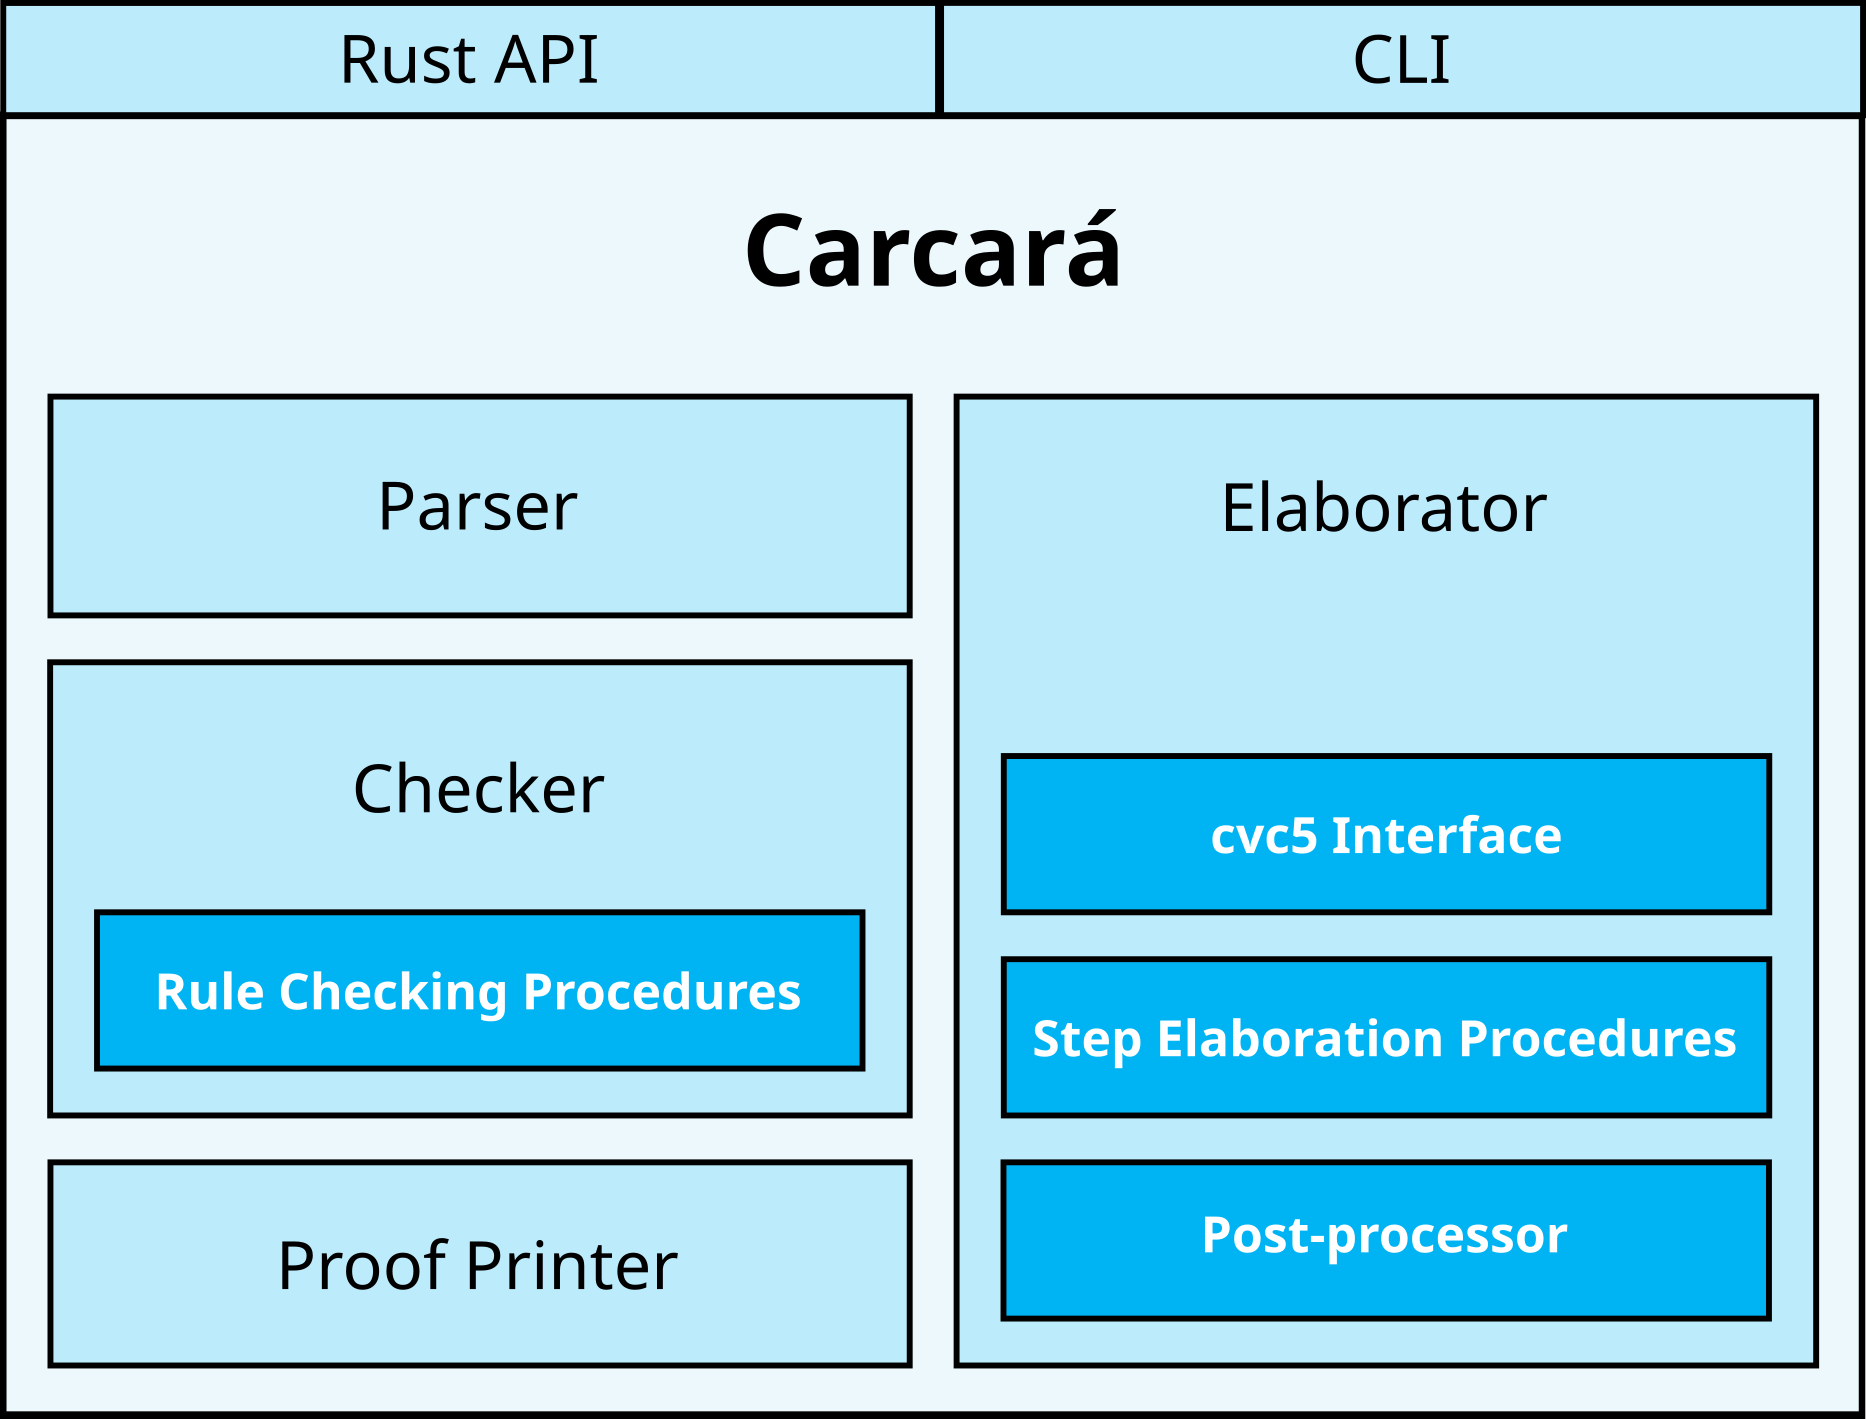
\includegraphics[height=0.6\textheight]{images/architecture.png}
  \end{minipage}
\end{frame}

\section{Checking}

\begin{frame}[fragile]
  \frametitle{Checking Alethe proofs}
  \begin{minipage}[c][0.6 \textheight]{0.49 \textwidth}
  \begin{itemize}
    \item The first step in checking an Alethe proof is parsing it
    \vitem Carcara uses \textit{hash consing} when parsing terms
    \vitem The proof is represented internally by an array of proof commands
  \end{itemize}
  \end{minipage}
  \begin{minipage}{0.5 \textwidth}
    \vspace{-.35ex}
    \begin{minted}[autogobble, fontsize=\footnotesize, frame=single]{haskell}
      Proof [
        Assume {
          id: "h1",
          term: (forall ((x Int)) (> x 0)),
        },
        Assume {
          id: "h2",
          term: (not (forall ((y Int)) (> y 0))),
        },
        Subproof {
          args: [(y Int), (:= x y)]
          commands: [
            Step {
              id: "t3.t1",
              clause: [(= x y)],
              rule: "refl",
              premises: [],
            },
        ...
    \end{minted}
  \end{minipage}
\end{frame}

\begin{frame}
  \frametitle{Checking Alethe proofs}
  \begin{itemize}
    \item A checking procedure had to be implemented for each of the 90 rules
    currently in the Alethe format
    \vitem The presence of coarse-grained proof steps makes checking difficult
    \vitem We will take a detailed look into what are some of the challenges in
    checking Alethe proofs
  \end{itemize}
\end{frame}

\begin{frame}
  \frametitle{Checking \textit{assume} commands}
  \begin{itemize}
    \item An \texttt{assume} command must contain a term introduced in one of the
    original problem's \texttt{assert}s
    \vitem During parsing, the problem's assumptions are stored in a hash set
    \vitem In general, checking an \textit{assume} command amounts to accessing
    that hash set
  \end{itemize}
\end{frame}

\begin{frame}[fragile]
  \frametitle{Checking \textit{assume} commands}
  \begin{minipage}[c][0.45 \textheight]{0.55 \textwidth}
    \begin{itemize}
      \item However, the solver may implicitly reorder equalities when producing
      a proof
      \vitem This means an \texttt{assume} command may reference a problem premise
      while implicitly reordering an equality inside it
    \end{itemize}
  \end{minipage}
  \hfill
  \begin{minipage}{0.4 \textwidth}
    \begin{minted}[autogobble, fontsize=\footnotesize, frame=single, escapeinside=||]{smtlib2.py -x}
      (set-logic QF_UF)
      (declare-const a Bool)
      (declare-const b Bool)
      (assert (= a b))
      (assert |\colorbox{yellow}{(not (= b a))}|)
      (check-sat)
    \end{minted}
    \begin{minted}[autogobble, fontsize=\footnotesize, frame=single, escapeinside=||]{smtlib2.py -x}
      (assume h1 (= a b))
      (assume h2 |\colorbox{yellow}{(not (= a b))}|)
      (step t3 (cl) :rule resolution
          :premises (h1 h2))
    \end{minted}
  \end{minipage}
\end{frame}

\begin{frame}[fragile]
  \frametitle{Checking \textit{assume} commands}
  \begin{minipage}[c][0.55 \textheight]{0.55 \textwidth}
    \begin{itemize}
      \item In this case, the checker must iterate through all the premises and
      see if they are equal to the \texttt{assume} term, modulo the reordering
      of equalities
      \vitem This requires traversing the terms, possibly up to their depth
      \vitem We call this equality check a \textit{Polyequal} check
    \end{itemize}
  \end{minipage}
  \hfill
  \begin{minipage}{0.4 \textwidth}
    \begin{minted}[autogobble, fontsize=\footnotesize, frame=single, escapeinside=||]{smtlib2.py -x}
      (set-logic QF_UF)
      (declare-const a Bool)
      (declare-const b Bool)
      (assert (= a b))
      (assert |\colorbox{yellow}{(not (= b a))}|)
      (check-sat)
    \end{minted}
    \begin{minted}[autogobble, fontsize=\footnotesize, frame=single, escapeinside=||]{smtlib2.py -x}
      (assume h1 (= a b))
      (assume h2 |\colorbox{yellow}{(not (= a b))}|)
      (step t3 (cl) :rule resolution
          :premises (h1 h2))
    \end{minted}
  \end{minipage}
\end{frame}

\begin{frame}[fragile]
  \frametitle{Checking linear arithmetic steps}
  \begin{itemize}
    \item The \texttt{la\_generic} rule models linear arithmetic reasoning
    \vitem For example, consider this \texttt{la\_generic} step:
    \begin{minted}[autogobble, fontsize=\footnotesize, frame=single]{smtlib2.py -x}
      (step t1
          (cl (<= (- x) 1) (<= (+ (* 2 x) (* (- 3) y)) 2) (<= y (- 1)))
          :rule la_generic :args (2 1 3))
    \end{minted}
    \vitem It introduces the following tautology:
    $$(-x \leq 1) \lor (2x - 3y \leq 2) \lor (y \leq -1)$$
  \end{itemize}
\end{frame}

\begin{frame}[t, fragile]
  \frametitle{Checking linear arithmetic steps}
  \begin{minted}[autogobble, fontsize=\footnotesize, frame=single]{smtlib2.py -x}
    (step t1
        (cl (<= (- x) 1) (<= (+ (* 2 x) (* (- 3) y)) 2) (<= y (- 1)))
        :rule la_generic :args (2 1 3))
  \end{minted}
  \begin{itemize}
    \item Checking that this clause is true is equivalent to proving that its
    negation, the following three inequalites, are contradictory
  \end{itemize}
  \begin{align*}
    -x &> 1\tag{a}\\
    2x - 3y &> 2\tag{b}\\
    y &> -1\tag{c}
  \end{align*}
\end{frame}
\addtocounter{framenumber}{-1}

\begin{frame}[t, fragile]
  \frametitle{Checking linear arithmetic steps}
  \begin{minted}[autogobble, fontsize=\footnotesize, frame=single, escapeinside=||]{smtlib2.py -x}
    (step t1
        (cl (<= (- x) 1) (<= (+ (* 2 x) (* (- 3) y)) 2) (<= y (- 1)))
        :rule la_generic |\colorbox{yellow}{:args (2 1 3)}|)
  \end{minted}
  \begin{itemize}
    \item Since \texttt{la\_generic} steps provide the needed coefficients as
    arguments, checking them is simple
    \vitem Computing $2 \cdot (a) + 1 \cdot (b) + 3 \cdot (c)$, we get $0 > 1$,
    so the step must be true
  \end{itemize}
  \begin{align*}
    -x &> 1\tag{a}\\
    2x - 3y &> 2\tag{b}\\
    y &> -1\tag{c}
  \end{align*}
\end{frame}

\begin{frame}[fragile]
  \frametitle{Checking linear arithmetic steps}
  \begin{itemize}
    \item The \texttt{lia\_generic} rule is very similar to
    \texttt{la\_generic}, but it does not provide the coefficients as arguments:
    \begin{minted}[autogobble, fontsize=\footnotesize, frame=single]{smtlib2.py -x}
      (step t1
          (cl (<= (- x) 1) (<= (+ (* 2 x) (* (- 3) y)) 2) (<= y (- 1)))
          :rule lia_generic)
    \end{minted}
    \vitem In this case, the checker would need to search for the coefficients,
    which is an NP-hard problem
    \vitem Instead, occurences of this rule are not checked, and are considered
    holes by Carcara
  \end{itemize}
\end{frame}

\section{Elaboration}

\begin{frame}
  \frametitle{Proof elaboration}
  \begin{itemize}
    \item There are many rules in Alethe which allow very coarse-grained steps
    \vitem By breaking them down into smaller, finer-grained steps, we can
    produce a proof that is easier to check and contains less holes
    \vitem Carcara implements elaboration procedures for a few important rules
  \end{itemize}
\end{frame}

\begin{frame}[fragile]
  \frametitle{A motivating example: transitivity}
  \begin{itemize}
    \item In Alethe, \texttt{eq\_transitive} is one of the rules that reasons
    about the transitivity of equality
    \vitem In general, a step of this rule looks like this:
    \begin{minted}[autogobble, fontsize=\footnotesize, frame=single]{smtlib2.py -x}
      (step t1 (cl (not (= a b)) (not (= b c)) (not (= c d)) (= a d)) :rule eq_transitive)
    \end{minted}
    \vitem In a more natural notation, it introduces the tautology:
    $$(a \neq b) \lor (b \neq c) \lor (c \neq d) \lor (a = d)$$
  \end{itemize}
\end{frame}

\begin{frame}[fragile]
  \frametitle{A motivating example: transitivity}
  \begin{itemize}
    \item However, the specification of this rule is very permissive
    \begin{itemize}
      \item The order of the transitive chain may be shuffled
      \item Each negated equality may also be flipped
    \end{itemize}
    \vitem Therefore, the following is also a valid \texttt{eq\_transitive}
    step:
    \begin{minted}[autogobble, fontsize=\footnotesize, frame=single]{smtlib2.py -x}
      (step t1 (cl (not (= b a)) (not (= c d)) (not (= c b)) (= a d)) :rule eq_transitive)
    \end{minted}
    \vitem This means that checking \texttt{eq\_transitive} is in general quadratic on
    the length of the clause (instead of linear)
  \end{itemize}
\end{frame}

\begin{frame}
  \frametitle{Elaborating \texttt{eq\_transitive}}
  \begin{itemize}
    \item A possible elaboration procedure for \texttt{eq\_transitive} might
    change the clause to ``unshuffle'' the transitive chain, and ``unflip'' the
    needed equalities
    \vitem However, steps later in the proof may refer to the
    \texttt{eq\_transitive} step as premise, so we can't just change the
    conclusion caluse
    \vitem Instead, we must also add  steps that reconstruct the original
    clause, so that it can still be referenced further down in the proof
  \end{itemize}
\end{frame}

\begin{frame}[fragile]
  \frametitle{Elaborating \texttt{eq\_transitive}}
  \begin{itemize}
    \item Here is an example \texttt{eq\_transitive} step:
    \begin{minted}[autogobble, fontsize=\footnotesize, frame=single]{smtlib2.py -x}
      (step t1 (cl (not (= b a)) (not (= c d)) (not (= c b)) (= a d)) :rule eq_transitive)
    \end{minted}
    \vitem ...and here is its elaboration:
    \begin{minted}[autogobble, fontsize=\footnotesize, frame=single]{smtlib2.py -x}
      (step t1.t1 (cl (not (= a b)) (not (= b c)) (not (= c d)) (= a d)) :rule eq_transitive)
      (step t1.t2 (cl (not (= b a)) (= a b)) :rule eq_symmetric)
      (step t1.t3 (cl (not (= c b)) (= b c)) :rule eq_symmetric)
      (step t1.t4 (cl (not (= c d)) (= a d) (not (= b a)) (not (= c b)))
          :rule resolution :premises (t1.t1 t1.t2 t1.t3))
      (step t1 (cl (not (= b a)) (not (= c d)) (not (= c b)) (= a d))
          :rule reordering :premises (t1.t4))
    \end{minted}
    \vitem The new \texttt{eq\_transitive} step, \texttt{t1.t1}, is now easy to
    check, and the step \texttt{t1} still has the same conclusion clause
  \end{itemize}
\end{frame}

\begin{frame}
  \frametitle{Removing the implicit reordering of equalities}
  \begin{itemize}
    \item As was mentioned earlier, SMT solvers may implicitly reorder
    equalities when producing Alethe proofs
    \vitem This makes checking more complicated and less efficient
    \vitem An elaboration procedure was also developed to remove this implicit
    transformation
  \end{itemize}
\end{frame}

\begin{frame}[fragile]
  \frametitle{Removing the implicit reordering of equalities}
  \begin{itemize}
    \item For example, consider the following SMT problem, and its corresponding
    proof:
    \begin{minipage}[t]{0.35 \textwidth}
      \begin{minted}[autogobble, fontsize=\footnotesize, frame=single]{smtlib2.py -x}
        (set-logic QF_UF)
        (declare-const a Bool)
        (declare-const b Bool)
        (assert (= a b))
        (assert (not (= b a)))
        (check-sat)
      \end{minted}
    \end{minipage}
    \hfill
    \begin{minipage}[t]{0.6 \textwidth}
      \begin{minted}[autogobble, fontsize=\footnotesize, frame=single]{smtlib2.py -x}
        (assume h1 (= a b))
        (assume h2 (not (= a b)))
        (step t3 (cl) :rule resolution :premises (h1 h2))
      \end{minted}
    \end{minipage}
    \vitem The proof would be simpler to check if \texttt{h2} was instead
    \texttt{(assume h2 (not (= b a)))}
    \vitem But \texttt{t3} uses \texttt{h2} as a premise, so we can't just
    change it --- like before, we also need to reconstruct the original
    conclusion
  \end{itemize}
\end{frame}

\begin{frame}[fragile]
  \frametitle{Removing the implicit reordering of equalities}
  \begin{itemize}
    \begin{minted}[autogobble, fontsize=\footnotesize, frame=single]{smtlib2.py -x}
      (assume h1 (= a b))
      (assume h2 (not (= a b)))
      (step t3 (cl) :rule resolution :premises (h1 h2))
    \end{minted}
    \vitem This is the correct elaboration of the proof:
    \begin{minted}[autogobble, fontsize=\footnotesize, frame=single]{smtlib2.py -x}
      (assume h1 (= a b))
      (assume h2 (not (= b a)))
      (step h2.t1 (cl (= (= b a) (= a b))) :rule equiv_simplify)
      (step h2.t2 (cl (= (not (= b a)) (not (= a b)))) :rule cong :premises (h2.t1))
      (step h2.t3 (cl (not (not (= b a))) (not (= a b))) :rule equiv1 :premises (h2.t2))
      (step h2.t4 (cl (not (= a b))) :rule resolution :premises (h2 h2.t3))
      (step t3 (cl) :rule resolution :premises (h1 h2.t4))
    \end{minted}
    \vitem Now \texttt{h2} refers to the premise as it appeared in the original
    problem, and the added steps reconstruct the original \texttt{h2} conclusion
    \vitem The step \texttt{t3}, that used to reference \texttt{h2}, now
    references \texttt{h2.t4}
  \end{itemize}
\end{frame}

\begin{frame}
  \frametitle{Removing \texttt{lia\_generic} holes}
  \begin{itemize}
    \item As was seen before, \texttt{lia\_generic} steps are very hard to
    check, and are considered holes by Carcara
    \vitem We developed an elaboration procedure that uses an SMT solver to
    expand these steps into finer-grained steps
    \vitem Conceivably this could use any solver that can read SMT-LIB, solve
    the linear integer arithmetic problem, and produce an Alethe proof
  \end{itemize}
\end{frame}

\begin{frame}[fragile]
  \frametitle{Removing \texttt{lia\_generic} holes}
  \begin{minipage}[c][0.6 \textheight]{0.65 \textwidth}
    \begin{itemize}
      \item In general, a \texttt{lia\_generic} step concludes a clause of
      negated inequalities $\neg l_1 \lor \cdots \lor \neg l_n$
      \vitem We generate an SMT instance that asserts the negation of this
      clause, that is, $l_1 \land \cdots \land l_n$
      \vitem A proof of the unsatisfiability of this SMT instance is also a
      proof of the validity of the \texttt{lia\_generic} step
    \end{itemize}
  \end{minipage}
  \hfill
  \begin{minipage}[c]{0.3 \textwidth}
    \begin{minted}[autogobble, fontsize=\footnotesize, frame=single]{smtlib2.py -x}
      (step t1 (cl
          (not l1)
          (not l2)
          ...
          (not ln)
      ) :rule lia_generic)
    \end{minted}
    $$\downarrow$$
    \begin{minted}[autogobble, fontsize=\footnotesize, frame=single]{smtlib2.py -x}
      (assert l1)
      (assert l2)
      ...
      (assert ln)
      (check-sat)
      (get-proof)
    \end{minted}
  \end{minipage}
\end{frame}

\begin{frame}[fragile]
  \frametitle{Removing \texttt{lia\_generic} holes}
  \begin{itemize}
    \item Now, Carcara sends this SMT instance to cvc5 and asks for an Alethe
    proof
    \vitem If one is provided before a timeout, it is inserted in the place of
    the \texttt{lia\_generic} step
  \end{itemize}
  \vfill
  \begin{minted}[autogobble, fontsize=\footnotesize, frame=single]{smtlib2.py -x}
    (step t1 (cl (not l1) (not l2) ... (not ln)) :rule lia_generic)
  \end{minted}
  $$\downarrow$$
  \begin{minted}[autogobble, fontsize=\footnotesize, frame=single]{smtlib2.py -x}
    (anchor :step t1.tm+1)
      (assume t1.h1 l1)                 ;
      ...                               ;
      (assume t1.hn ln)                 ; proof generated by cvc5
      ...                               ;
      (step t1.tm (cl false) :rule ...) ;
    (step t1.tm+1 (cl (not l1) ... (not ln) false) :rule subproof)
    (step t1.tm+2 (cl (not false)) :rule false)
    (step t1 (cl (not l1) ... (not ln)) :rule resolution :premises (t1.tm+1 t1.tm+2))
  \end{minted}
\end{frame}

\section{Evaluation}

\begin{frame}
  \frametitle{Experimental setup}
  \begin{itemize}
    \item We used the veriT SMT solver to generate Alethe proofs from all
    problems in the SMT-LIB benchmark library
    \vitem This resulted in a 92 GB set of 39,229 proofs
    \vitem Most proofs are small (under 1 MB), but some can be very large
    \begin{itemize}
      \item 14 proofs are over 1 GB, and the largest has 4.5 GB
    \end{itemize}
  \end{itemize}
\end{frame}

\begin{frame}
  \frametitle{Proof checking}
  \begin{itemize}
    \item We used Carcara to check all proofs in the benchmark set
    \vitem 378 proofs had checking failures, but they were all due to incorrect
    steps caused by bugs in the solver
    \vitem In aggregate, checking was 4.69 times faster than solving
  \end{itemize}
\end{frame}

\begin{frame}
  \frametitle{Proof checking}
  \begin{minipage}{0.31 \textwidth}
    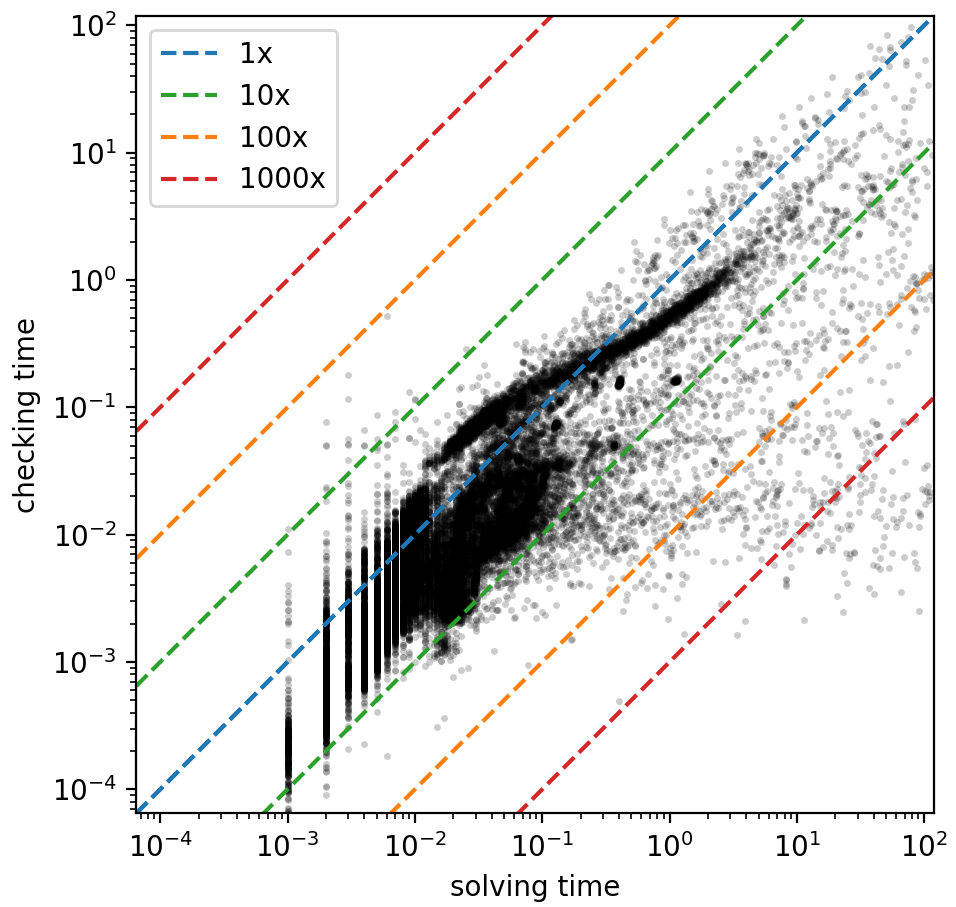
\includegraphics[height=0.75 \textheight]{images/solving-checking.png}
    \hfill
  \end{minipage}
  \begin{minipage}{0.68 \textwidth}
    \hfill
    \notsotiny
    \begin{tabular}{l|r|r|r|r}
      \toprule
      \textbf{Logic} & \textbf{Problems} & \textbf{Solving (s)} &
          \textbf{Checking (s)} & \textbf{Ratio} \\ \midrule
      QF\_LIA & 1018 & 5975 & 742 & 8.05 \\
      QF\_UF & 4180 & 3857 & 1881 & 2.05 \\
      QF\_LRA & 537 & 3629 & 258 & 14.03 \\
      UFLIA & 7221 & 3547 & 136 & 26.05 \\
      QF\_IDL & 609 & 3316 & 2240 & 1.48 \\
      UF & 2885 & 2858 & 30 & 92.35 \\
      QF\_UFLIA & 167 & 1194 & 4 & 254.41 \\
      AUFLIA & 2135 & 1094 & 12 & 87.53 \\
      QF\_RDL & 81 & 620 & 123 & 5.04 \\
      QF\_UFIDL & 66 & 396 & 87 & 4.53 \\
      AUFLIRA & 19200 & 248 & 144 & 1.73 \\
      QF\_UFLRA & 415 & 141 & 65 & 2.18 \\
      QF\_ALIA & 16 & 0.79 & 1.39 & 0.57 \\
      UFIDL & 55 & 0.54 & 0.66 & 0.82 \\
      QF\_AUFLIA & 256 & 0.34 & 0.11 & 3.04 \\
      UFLRA & 10 & 0.02 & 0.01 & 3.05 \\
      \midrule
      Total: & 38851 & 26882.93 & 5729.39 & 4.69 \\
      \bottomrule
    \end{tabular}
  \end{minipage}
\end{frame}

\begin{frame}
  \frametitle{Proof checking}
  \begin{minipage}{0.64 \textwidth}
    \centering
    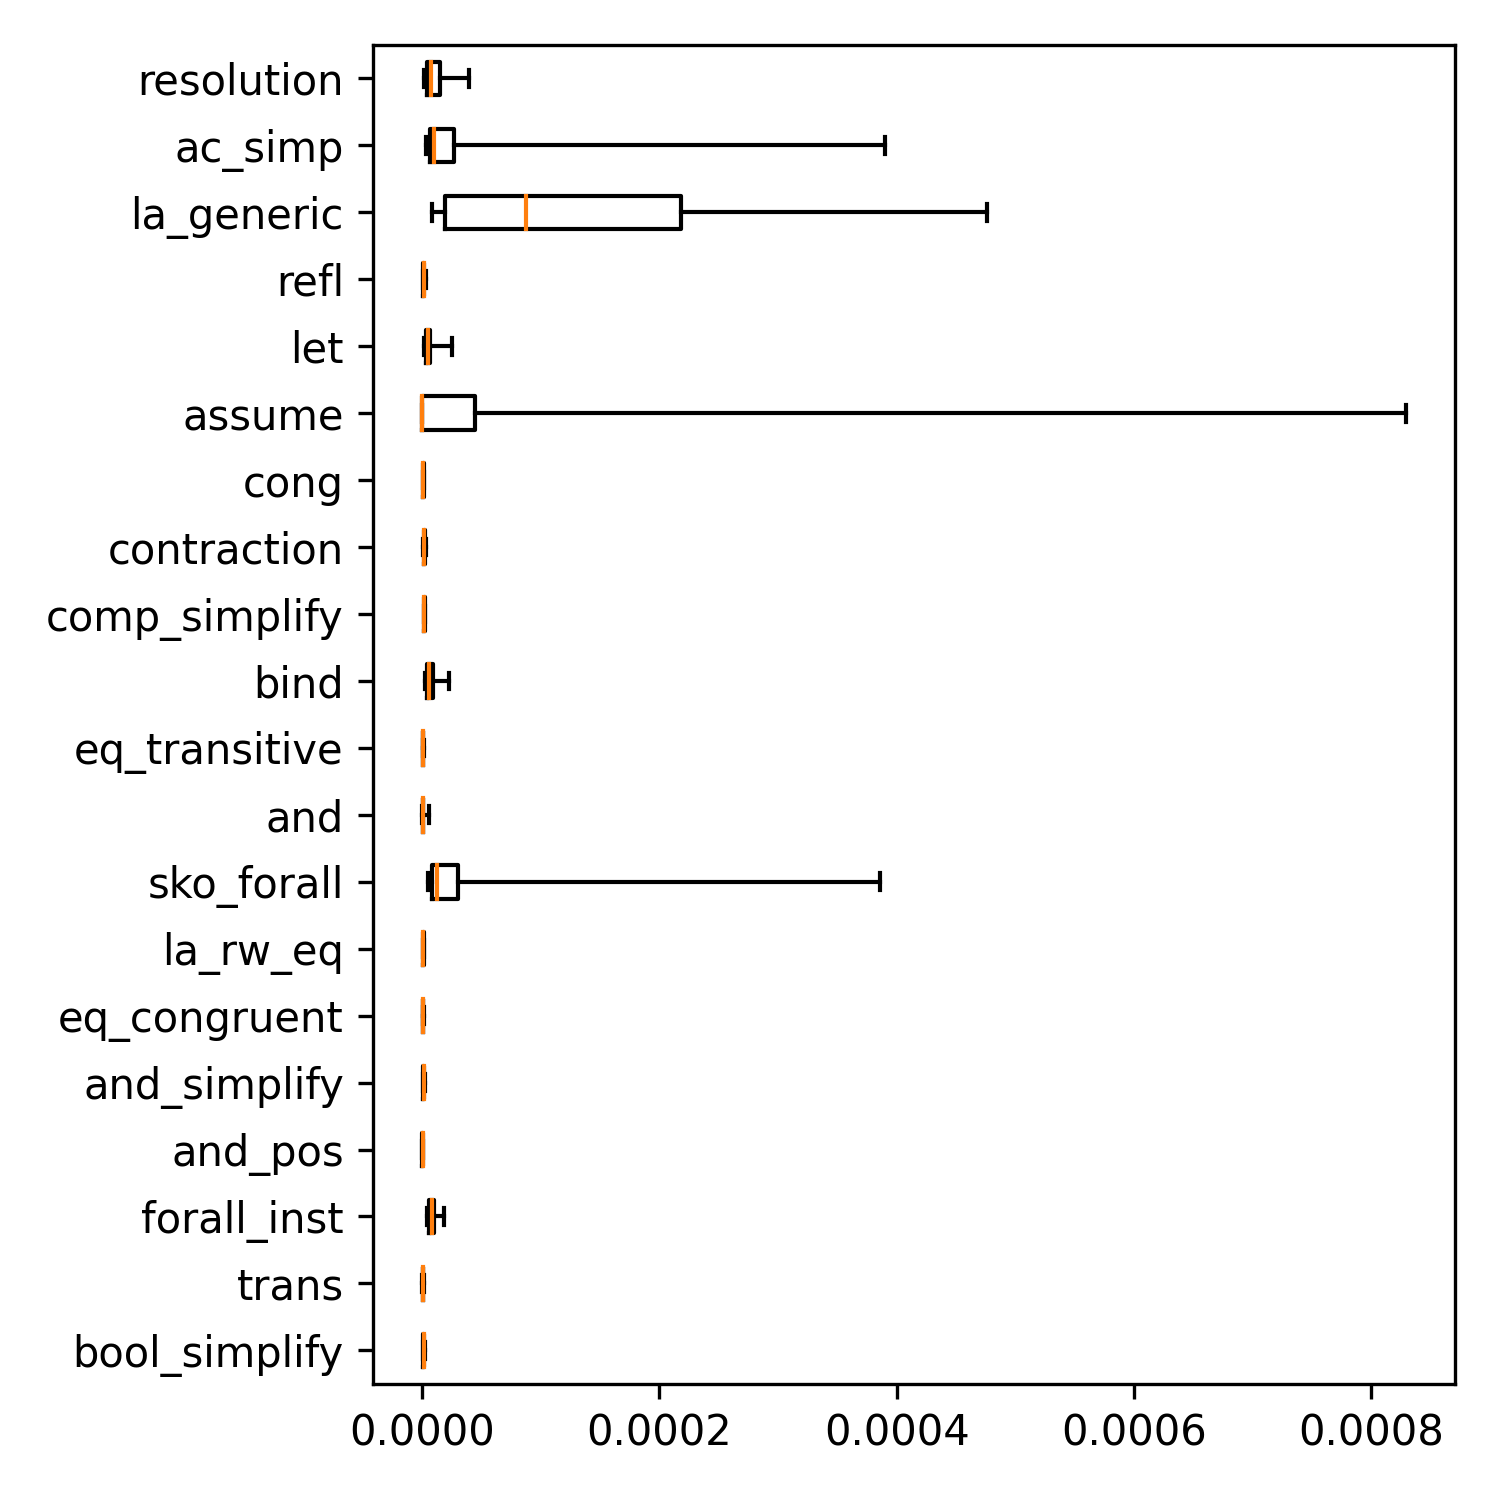
\includegraphics[height=0.9\textheight]{images/by-rules-boxplot.png}
  \end{minipage}
  \hfill
  \begin{minipage}[c][0.8 \textheight]{0.3 \textwidth}
    \begin{itemize}
      \item \texttt{resolution} and \texttt{refl} are simple to check, but very
      frequent
      \vitem \texttt{la\_generic} and \texttt{ac\_simp} are much less frequent,
      but checking them is more expensive
      \vitem Note how \texttt{assume} has some very expensive worst cases
      \vfill
    \end{itemize}
  \end{minipage}
\end{frame}

\begin{frame}
  \frametitle{Proof elaboration}
  \begin{itemize}
    \item We also used Carcara to elaborate all proofs in the benchmark set
    \vitem Then, we used it to check the elaborated proofs, and compared the
    performance
    \vitem Overall, proof elaboration sped up checking time by 6\%
    \vitem On the other hand, parsing time increased, such that the overall
    runtime is virtually the same
  \end{itemize}
\end{frame}

\begin{frame}
  \frametitle{Impact of proof elaboration by rule}
  \centering
  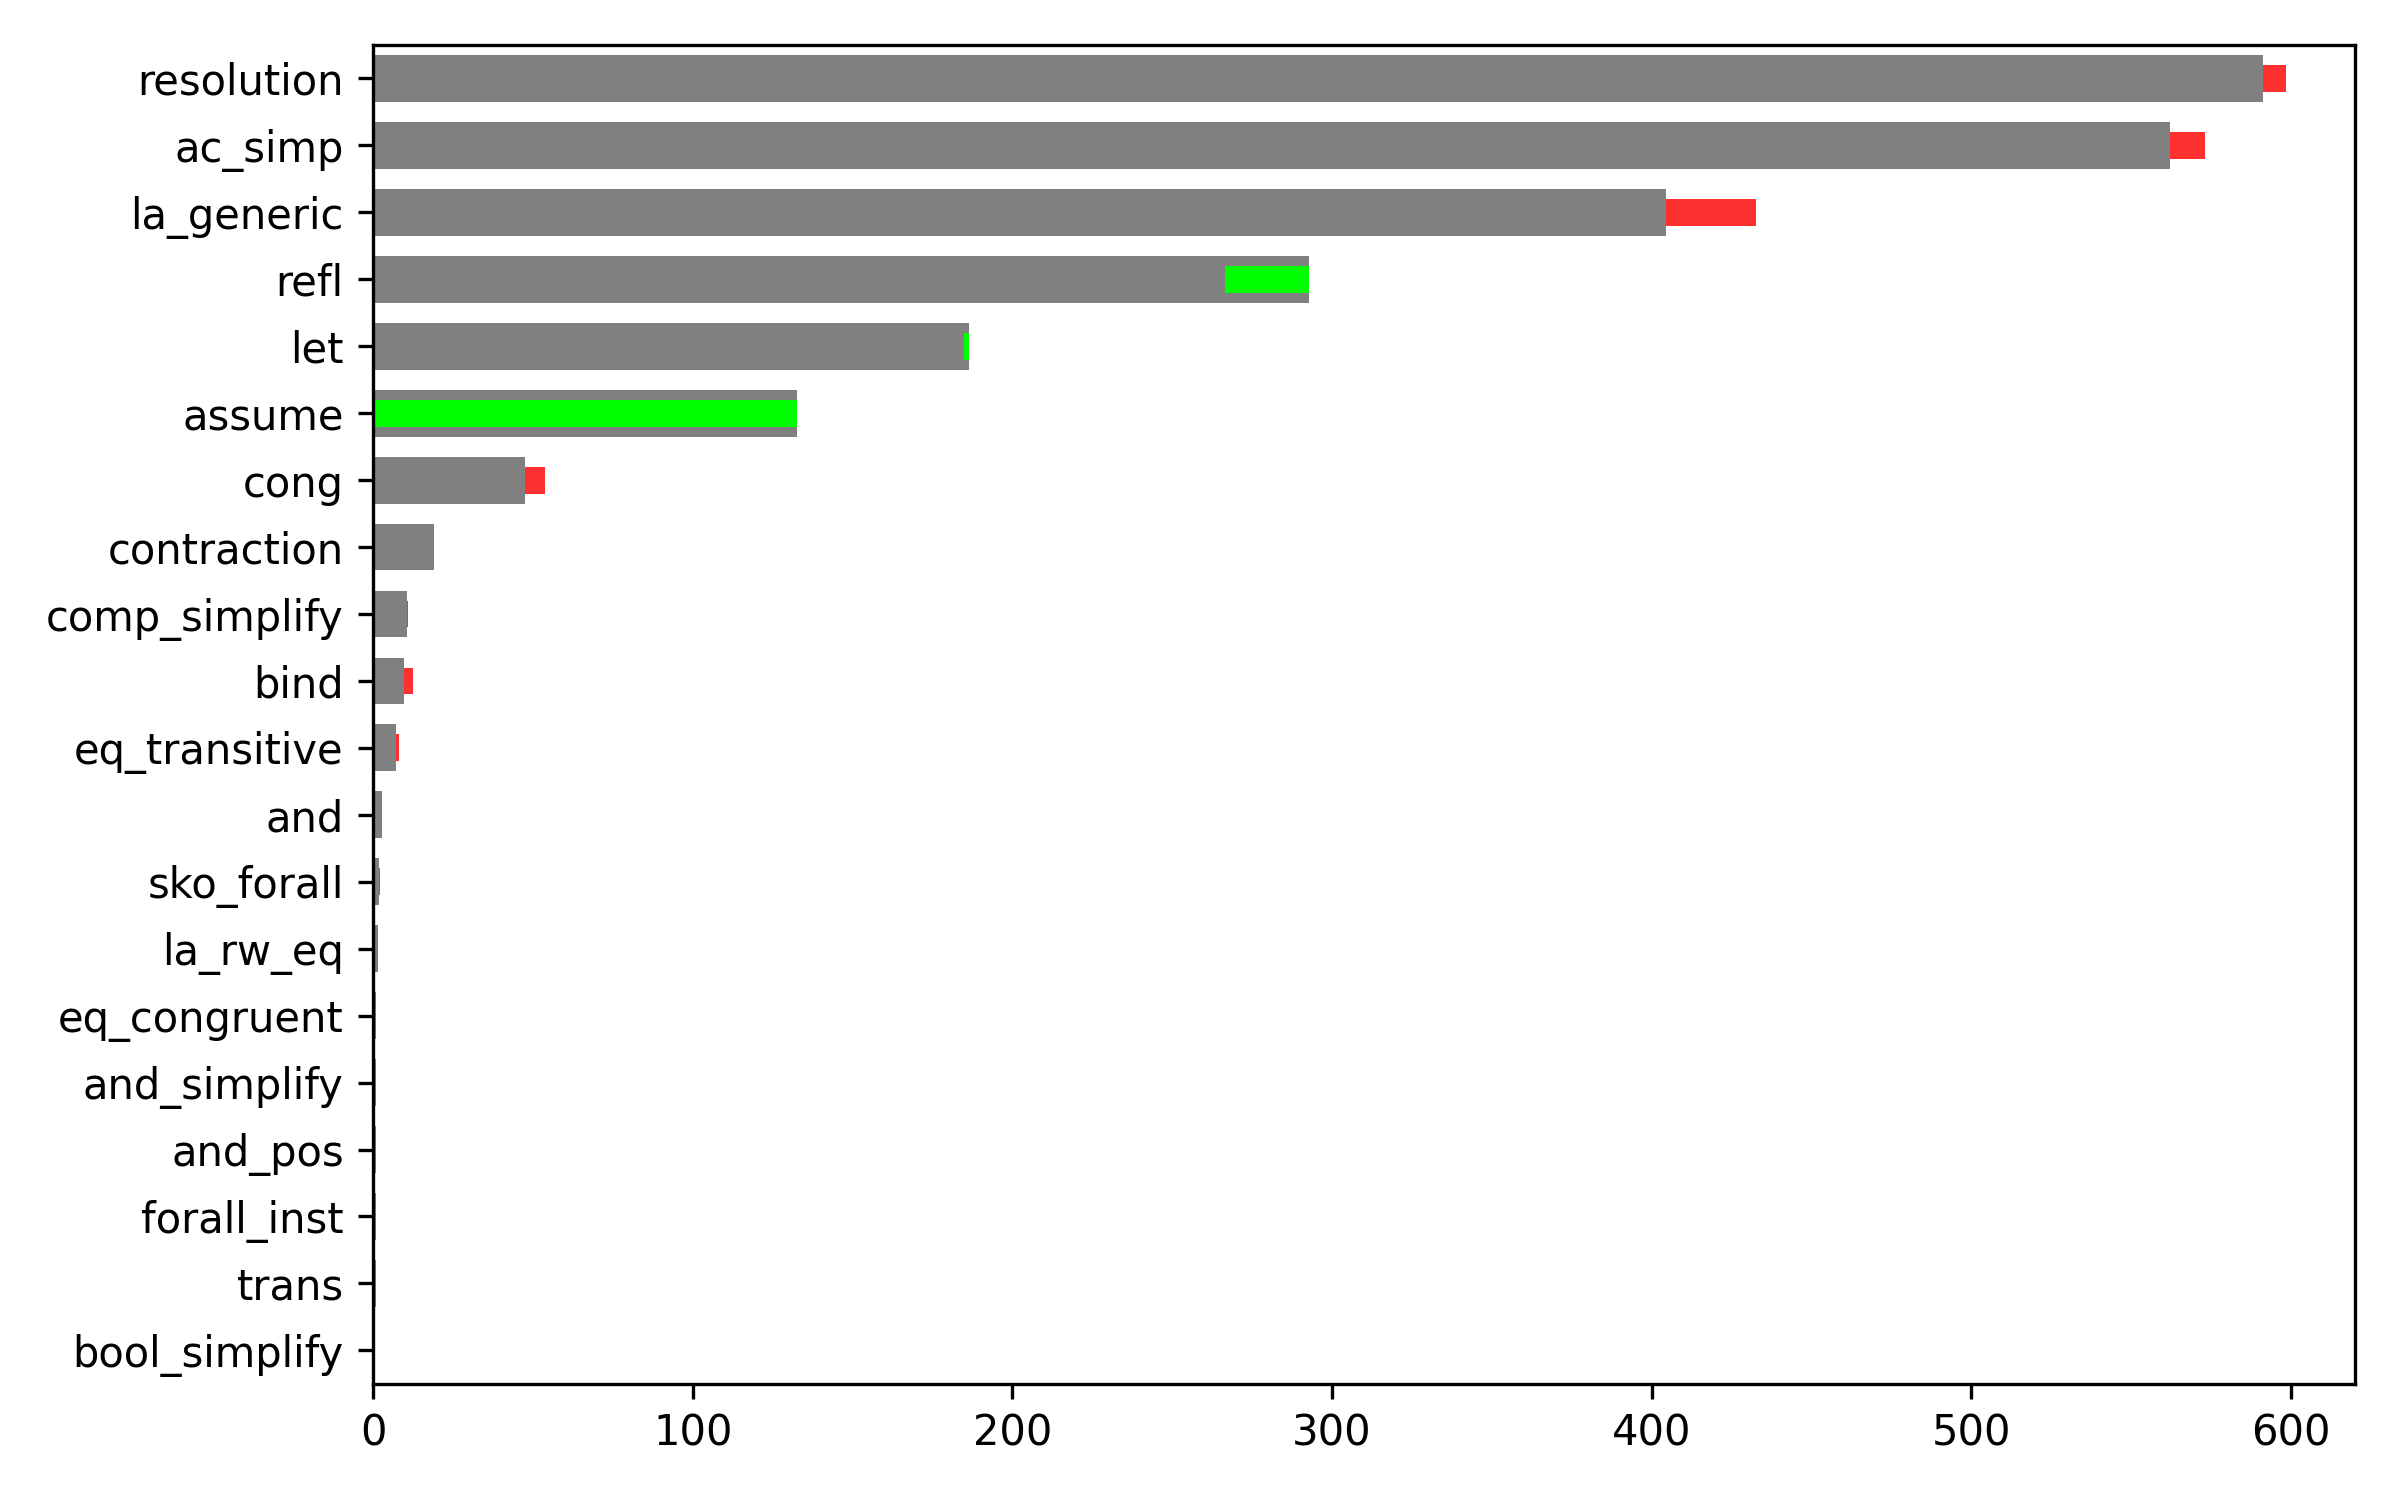
\includegraphics[height=0.85\textheight]{images/by-rules-comp.png}
\end{frame}

\begin{frame}
  \frametitle{Elaboration of \texttt{lia\_generic} holes}
  \begin{itemize}
    \item We also ran experiments with elaboration of \texttt{lia\_generic}
      enabled
    \vitem In the benchmark set, there were 276 proofs, with a total of 127k
    \texttt{lia\_generic} steps
    \begin{itemize}
      \item 15 proofs were discarded due to limitations in cvc5's Alethe support
      \item Carcara timed out on 13 proofs
    \end{itemize}
    \vitem We used a 30 minute timeout for Carcara, and a 30 second timeout for
    cvc5 for each \texttt{lia\_generic} step
  \end{itemize}
\end{frame}

\begin{frame}
  \frametitle{Elaboration of \texttt{lia\_generic} holes}
  \begin{itemize}
    \item Of the remaining 261 proofs, 82 still cointained \texttt{lia\_generic}
      holes after elaboration
    \begin{itemize}
      \item In some cases, caused by cvc5 time outs, and in others by the cvc5
        generated proof itself containing \texttt{lia\_generic} steps
    \end{itemize}
    \vitem All of the proofs contained holes caused by unsupported cvc5 rewriting steps
    \vitem However, these holes are simpler and less worrying than the original
    ones
  \end{itemize}
\end{frame}

\section{Demo!}

\begin{frame}
  \frametitle{Conclusion}

  \begin{itemize}
    \item Good performance in checking SMT proofs
    \vitem Elaboration has potential when used as a bridge between solvers and
    proof assistants
    \vitem Carcara is already being used by SMT solver delevopers!
    \vitem Future work
    \begin{itemize}
      \item Parallelization of proof checking
      \item Proof compression
      \item Support for new theories: strings, bitvectors
      \item Proof translation into other formats: Dedukti
    \end{itemize}
  \end{itemize}
\end{frame}

\maketitle

\end{document}

%%% Local Variables:
%%% mode: latex
%%% TeX-master: t
%%% End:
